\begin{frame}[fragile]{Tutorial: n-site states with MPS}

\begin{columns}

\begin{column}{4.5cm}

\begin{onlyenv}<1->
\begin{lstlisting}[language=JuliaLocal, style=julia, mathescape, basicstyle=\small]
  n = 30
  i = [Index(2, "S=1/2")
        for j in 1:n]

  Zp = MPS(i, "Z+")
  Zm = MPS(i, "Z-")

  maxlinkdim(Zp)
\end{lstlisting}
\end{onlyenv}

\end{column}

\begin{column}{5.5cm}

\begin{onlyenv}<1-1>
$n$-site state \\
~\\
~\\
$|Z+Z+\dots Z+\rangle$ \\
$|Z-Z-\dots Z-\rangle$ \\
~\\
1 (product state)
\end{onlyenv}

\begin{onlyenv}<2->
\vspace*{0.0cm}
\begin{center}

\includegraphics[width=0.15\textwidth]{
  slides/assets/in.png
} \\
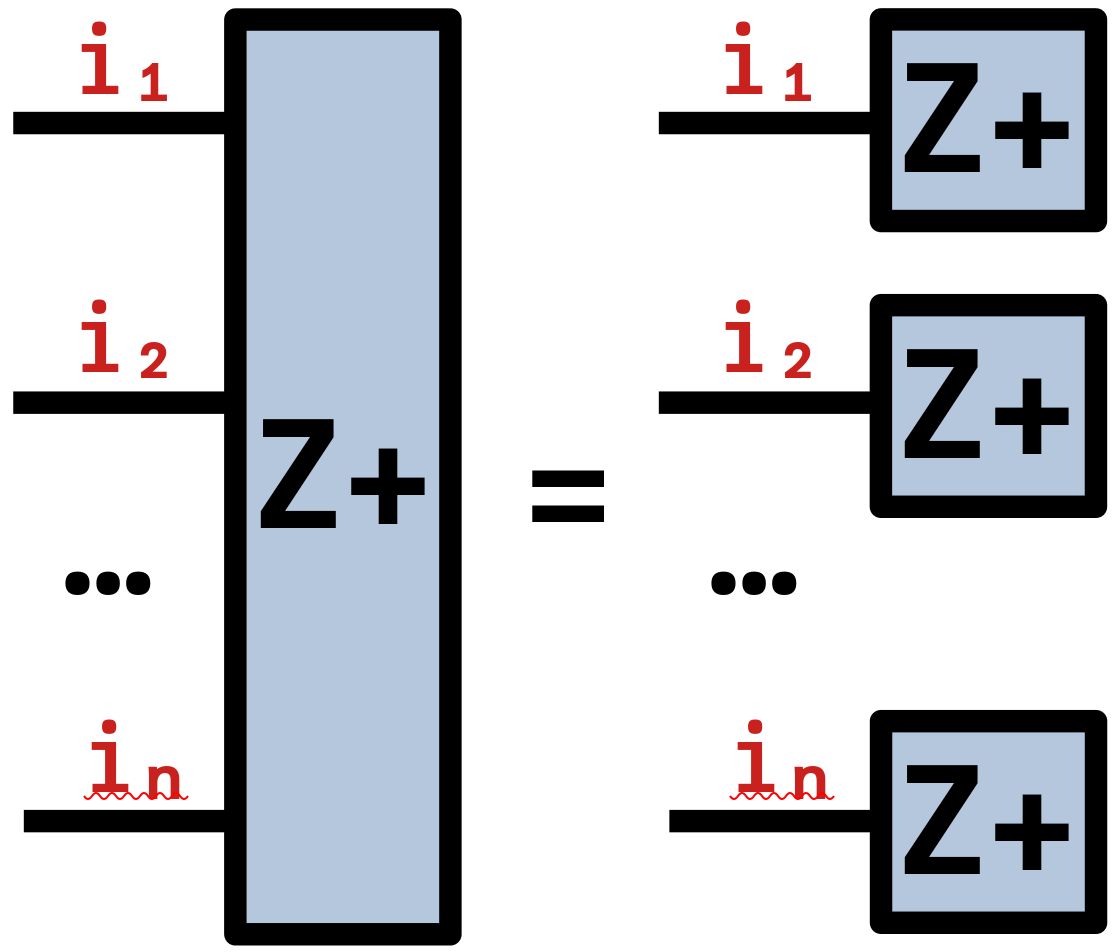
\includegraphics[width=0.45\textwidth]{
  slides/assets/Zpn.png
} \ \ 
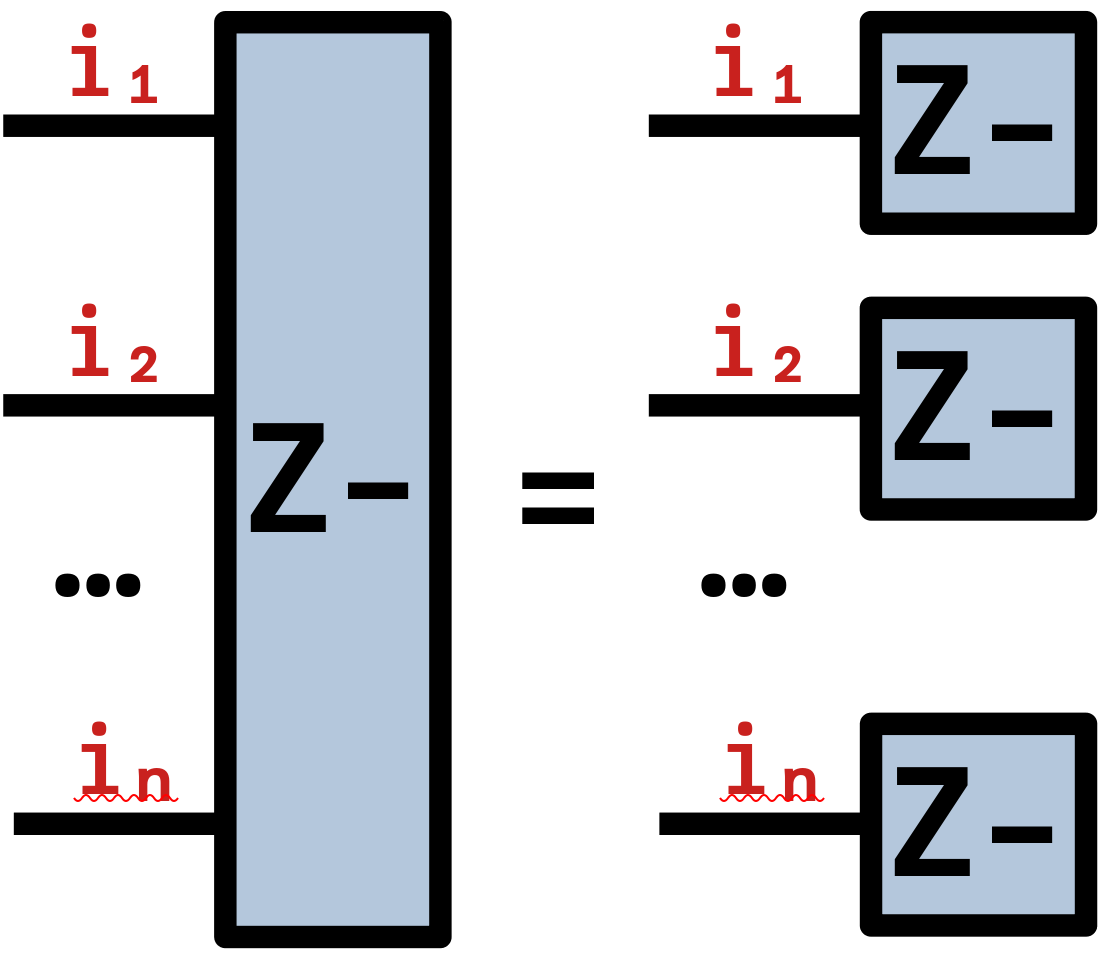
\includegraphics[width=0.45\textwidth]{
  slides/assets/Zmn.png
}
\end{center}
\vspace*{0.0cm}
\end{onlyenv}

\end{column}

\end{columns}

\end{frame}
